%%%%%%%%%%%%%%%%%%%%%%%%%%%%%%%
%%%%%%%%%% Notes/todo %%%%%%%%%

%% setup as two boxed with ideal/full data and observed

%% fix x vs (w,a)



%%%%%%%%%%%%%%%%%%%%%%%%%%%%%%%%%%%%%%%%% 
% a0poster Portrait Poster 
% LaTeX Template
% with University Copenhagen logo
% Version 1.0 (22/06/13)
%
% Based on:
% The a0poster class was created by:
% Gerlinde Kettl and Matthias Weiser (tex@kettl.de)
% 
% This template has been downloaded from:
% http://www.LaTeXTemplates.com
%
%%%%%%%%%%%%%%%%%%%%%%%%%%%%%%%%%%%%%%%%%

%----------------------------------------------------------------------------------------
%	PACKAGES AND OTHER DOCUMENT CONFIGURATIONS
%----------------------------------------------------------------------------------------

\documentclass[a0,portrait]{a0poster}
\usepackage[utf8]{inputenc}

\usepackage{multicol} % This is so we can have multiple columns of text side-by-side
\columnsep=100pt % This is the amount of white space between the columns in the poster
\columnseprule=3pt % This is the thickness of the black line between the columns in the poster

\usepackage[svgnames]{xcolor} % Specify colors by their 'svgnames', for a full list of all colors available see here: http://www.latextemplates.com/svgnames-colors

\usepackage{times} % Use the times font
%\usepackage{palatino} % Uncomment to use the Palatino font

\usepackage{graphicx} % Required for including images
\graphicspath{{figures/}} % Location of the graphics files
\usepackage{booktabs} % Top and bottom rules for table
\usepackage[font=small,labelfont=bf]{caption} % Required for specifying captions to tables and figures
\usepackage{amsfonts, amsmath, amsthm, amssymb, dsfont} % For math fonts, symbols and environments
\usepackage{wrapfig} % Allows wrapping text around tables and figures
\definecolor{ku}{RGB}{144,26,30}
\definecolor{ku-yellow}{RGB}{255,249,25}

\usepackage[most]{tcolorbox}

\usepackage{prodint}

%% The following is used to counter the parskip
\usepackage{titlesec} 
\titlespacing*{\section}{0pt}{\baselineskip}{-.3em}

% \usepackage{titlesec} 
% \usepackage{xhfill}
% \newcommand\ruleafter[1]{#1~\xrfill[.7ex]{1pt}}
% \titleformat{\section}
%   {\Large\bfseries}{\thesection}{1em}{\ruleafter}


%% own commands
\newcommand*\diff{\mathop{}\!\mathrm{d}}
\newcommand{\midd}{\; \middle|\;}
\newcommand{\R}{\mathbb{R}}
\newcommand{\1}{\mathds{1}}
\DeclareMathOperator{\E}{\mathbb{E}} % expectation

 \usepackage{eso-pic}
               \newcommand\BackgroundIm{
               \put(66,-71){
               \parbox[b][\paperheight]{\paperwidth}{%
               \vfill
               \centering
               
\includegraphics[height=\paperheight,width=\paperwidth,
               keepaspectratio]{background2.pdf}%
               \vfill
             }}}
         %% 



         \begin{document}

         \AddToShipoutPicture{\BackgroundIm}          %% Slightly buggish...
         \begin{minipage}{\textwidth}         


%----------------------------------------------------------------------------------------
%	POSTER HEADER 
%----------------------------------------------------------------------------------------

% The header is divided into two boxes:
% The first is 75% wide and houses the title, subtitle, names, university/organization and contact information
% The second is 25% wide and houses a logo for your university/organization or a photo of you
% The widths of these boxes can be easily edited to accommodate your content as
% you see fit




\begin{minipage}[t]{1\linewidth} %{0.60\linewidth}
  % \vspace{9.5cm}
  \vspace{-.5cm}
  \Huge \color{ku} \textbf{Causal parameter estimation with right-censored data
    \\
    using the state learner} \color{Black}
   % \\[0.5cm] % Title
   % \huge\textit{A super learner for right-censored data}
   % \\[1cm]
   \\[3.5cm] 
   \begin{minipage}[t]{.5\linewidth}
     \Large \textbf{Anders Munch} \& \textbf{Thomas Gerds} \\[0.5cm] % Author(s)
     \Large \color{DarkSlateGray} Section of Biostatistics, University of
     Copenhagen
      % \flushright
      % \\[1em]
      % \large \textbf{Contact:} \texttt{a.munch@sund.ku.dk}% Email address
    \end{minipage}
  \end{minipage}

  \vspace{1cm}
  
% \begin{minipage}[t]{1\linewidth} %{0.60\linewidth}
%    \vspace{9.5cm} \Huge \color{ku} \textbf{Causal parameter estimation with
%      right-censored data using the state learner}
%    \color{Black}
%    % \\[0.5cm] % Title
%    % \huge\textit{A super learner for right-censored data}
%    % \\[2cm] % Subtitle
%    \vspace{0.5cm}
%    \setlength{\columnseprule}{0pt}
%    \begin{multicols}{2}
%    % \begin{minipage}[t]{.5\linewidth}
%       \Large \textbf{Anders Munch} \& \textbf{Thomas Gerds} \\[0.5cm] % Author(s)
%       \Large \color{DarkSlateGray} Section of Biostatistics
%       % , University of Copenhagen
%     % \end{minipage}
%     % \begin{minipage}[t]{.5\linewidth}
%     %   \color{black}

%       \vspace{1cm}

%       % \Large \textbf{Contact information}\\
%       \textbf{Contact:} \texttt{a.munch@sund.ku.dk}% Email address

%       \vfill\null
%       %\hrule
%       \columnbreak

%       \color{black}
%   \begin{abstract}
%     ... The super learner is a machine learning algorithm which combines a
%     library of prediction models into a meta learner based on cross-validated
%     loss. Unfortunately, the commonly used partial likelihood loss is not suited
%     for super learning, and inverse probability of censoring weighted loss
%     functions require a pre-specified estimator of the censoring distribution.
%     To relax this, we introduce the state learner, a new super learner for
%     survival analysis, which evaluates the loss based on the observed data
%     simultaneously using libraries of predictions models for the event(s) of
%     interest and the censoring distribution. We establish an oracle inequality
%     for the state learner and investigate its performance through numerical
%     experiments. We illustrate how the state learner allows us to estimate
%     causal effects in a competing risks setting without having to pre-specify
%     models for neither the cause-specific hazards of interest nor the censoring
%     distribution.
% \end{abstract}
% % \hrule
%   % \flushright
%   %   \Large \textbf{Contact information}\\
%   %   \texttt{a.munch@sund.ku.dk}% Email address
%   % \end{minipage}
% \end{multicols}
% \end{minipage}

  \vspace{3cm}

\begin{minipage}[t]{1\linewidth}
  
  \begin{multicols}{2}
    \setlength{\parskip}{.5em}
    \setlength{\parindent}{0em}



%----------------------------------------------------------------------------------------
%	ABSTRACT
%----------------------------------------------------------------------------------------

    \color{black}    

\begin{abstract}

  The super learner is a machine learning algorithm which combines a
  library of prediction models into a meta learner based on
  cross-validated loss.  We introduce the state learner, a new super
  learner for survival analysis, which evaluates the loss based on the
  observed data simultaneously using libraries of predictions models
  for the events of interest and the censoring distribution. We
  establish an oracle inequality for the state learner and investigate
  its performance through numerical experiments. We illustrate how the
  state learner allows us to estimate causal effects in a competing
  risks setting without having to prespecify models for neither the
  cause-specific hazard functions nor the censoring distribution.
\end{abstract}

%----------------------------------------------------------------------------------------
%	INTRODUCTION
%----------------------------------------------------------------------------------------



\section*{Motivation}

Super learning uses cross-validation to decides which estimators best
fit the data. In survival analysis the result of super learning can be
a risk prediction model. Targeted learning can integrate super
learning of nuisance parameters and provide valid post-selection
inference for causal parameters.

\begin{center}
  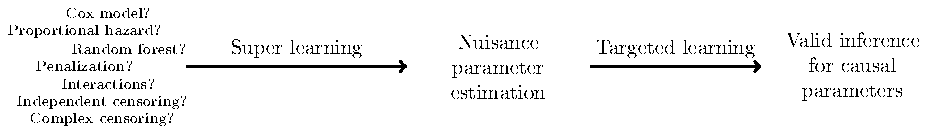
\includegraphics[width=1\linewidth]{motivation.pdf}
\end{center}

\section*{Problem statement}
\vspace{-.2em}
\setlength{\columnseprule}{0pt}
\setlength{\columnsep}{30pt}
\begin{multicols}{2}
  \begin{tcolorbox}[width=\linewidth,colframe=white, title={\center \textbf{Ideal data: \( \left(W,
      T^{0}, D^{0}, T^{1}, D^{1}\right) \sim Q \)}}, coltitle=black, colbacktitle=white]
\( W \in \mathcal{W} \subset \R^d \) is a vector of covariates,
\( T^{a} \in [0, \tau] \) is a counterfactual time to event variable under
treatment \( a \), and \( D^{a} \times \{1,2\} \) denotes the cause of the
event. The maximal length of followup is $\tau <\infty$.
\end{tcolorbox}

\begin{tcolorbox}[width=\linewidth,colframe=white, title={\center\textbf{
      Observed data: \( O= (W,
    A, \tilde T, \tilde D) \sim P \)}}, coltitle=black,
  colbacktitle=white]
  \( A \in {\{0,1\}} \) is a binary treatment administered in observed
  % (non-interventional)
  data. The pair \( (\tilde T, \tilde D) \) is the censored
  outcome variable, defined as \( \tilde T = T^a \wedge C^a \) and
  \( \tilde D^a = \1{\{T^a \leq C^a\}} D^a \), when \( A=a \), for some
  censoring time \( C^a \).
\end{tcolorbox}
\end{multicols}

\begin{multicols}{2}[{Targeted estimation of causal effects, such as the average treatment effect
    \begin{equation*}
      \Psi(Q) = 
      Q{
        \bigl(
          T^{1} \leq \tau, D^{1}=1
        \bigr)}-
      Q{\bigl(
          T^{0} \leq \tau, D^{0}=1
        \bigr)},
    \end{equation*}
    rely on estimators of the cause-specific cumulative hazard functions,
\begin{equation*}
  \Lambda_{j}(t \mid w, a) = \int_0^t\frac{  Q(T^a \in \diff s, D^a=j \mid W=w)}
  {Q(T^a \geq s \mid W=w)},
  \quad j \in \{1,2\},
\end{equation*}\vspace{-1em}}]
and the censoring probability. Assuming coarsening at random
\cite{gill1997coarsening,van2003unified}, the cause-specific hazard functions
and the censoring probability can be estimated based on samples from \( P \).
Many existing methods are available for this task, including the Nelson-Aalen
estimator, Cox models, random survival forests, Poisson regression, and neural
networks. % These methods will be
% valid under different assumptions.

A super learner can be used to data-adaptively select an estimator (called a
learner) from a library of candidates. Super learning uses cross-validation to
estimate and evaluate the performance of each learner in the library using a
given loss function. Our focus in this work is on how a super learner can assess
performance in a right-censored validation set without prespecification of an
estimator of the censoring probability.

\vfill\null\columnbreak

{\color{white}dummy}

  \begin{center}\vspace{-.5em}
    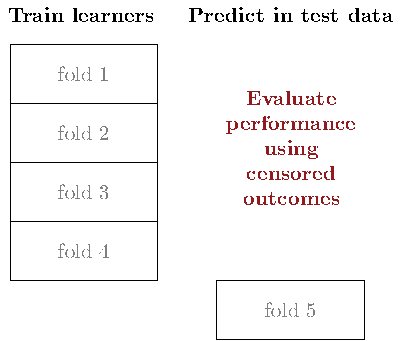
\includegraphics[width=1\linewidth]{cv-viz.pdf}
  \end{center}
  
\end{multicols}




% \vspace{5cm}

% \setlength{\columnseprule}{0pt}
% \begin{multicols}{2}


% In practice We observed censored data \( O = (W,A,\tilde T, \tilde D )\), where
% \( \tilde T = T \wedge C \) and \( \tilde D = \1{\{T \leq C\}} D \), for some
% censoring time \( C \).

% something
% In practice We observed censored data \( O = (W,A,\tilde T, \tilde D )\), where
% \( \tilde T = T \wedge C \) and \( \tilde D = \1{\{T \leq C\}} D \), for some
% censoring time \( C \).

% something
% In practice We observed censored data \( O = (W,A,\tilde T, \tilde D )\), where
% \( \tilde T = T \wedge C \) and \( \tilde D = \1{\{T \leq C\}} D \), for some
% censoring time \( C \).

% \vfill\null\columnbreak

%   \begin{center}\vspace{1cm}
%     
\includegraphics[width=1\linewidth]{placeholder}
%   \end{center}\vspace{1cm}

% \end{multicols}

\vspace{-2em}

\section*{Existing methods}

A commonly used loss function in survival analysis is the negative
partial log-likelihood loss. This loss is not perfectly suited for
super learning because many common survival estimators have infinite
loss in a hold out sample. This is illustrated in the figure below to
the left. Alternative methods such as inverse probability of censoring
weighting \cite{graf1999assessment,gonzalez2021stacked},
pseudo-observations \cite{andersen2003generalised,sachs2019ensemble},
and censoring unbiased transformations
\cite{steingrimsson2019censoring} rely on a prespecified estimator of
the censoring probability. This can lead to a circular reasoning as
illustrated in the figure below to the right. A recent proposal is to
iteratively estimate the survival and the censoring probabilities
\cite{westling2021inference}. However, no general theoretical guarantees
seem to exist for this procedure, and it has not yet been extended to
the situation with competing risks.

% \setlength{\columnseprule}{0pt}
% \setlength{\columnsep}{30pt}
% \begin{multicols}{2}
%   \begin{center}
%       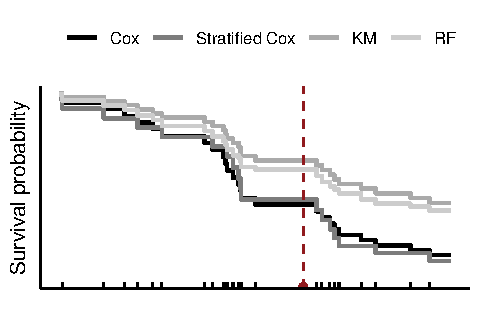
\includegraphics[width=.9\linewidth]{sl-hold-out-sample.pdf}
%     \end{center}
%     \begin{center}
%           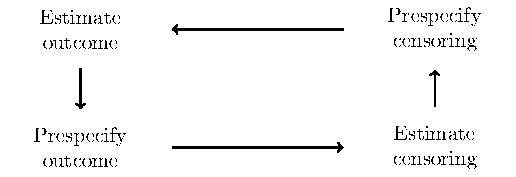
\includegraphics[width=1\linewidth]{ipcw-circle.pdf}
%     \end{center}
% \end{multicols}

\begin{minipage}[c]{0.5\linewidth}
  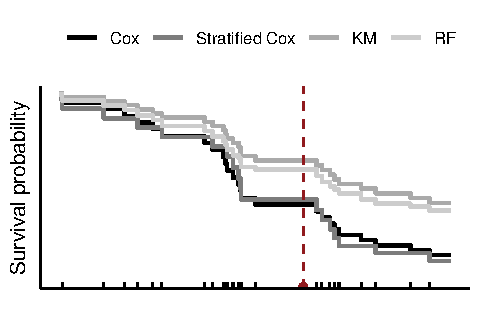
\includegraphics[width=.9\linewidth]{sl-hold-out-sample.pdf}
\end{minipage}
\begin{minipage}[c]{.5\linewidth}
\begin{center}
  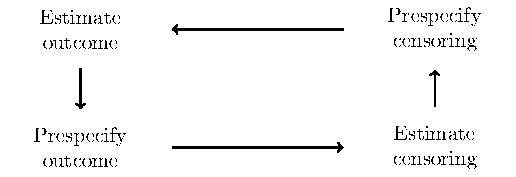
\includegraphics[width=1\linewidth]{ipcw-circle.pdf}
\end{center}
\end{minipage}


\vfill\null\columnbreak

% Parameters
% $\Psi \colon \mathcal{Q} \rightarrow \R$ such as
% \begin{align*}
%   \Psi_t(Q) & = \int_{\mathcal{W}}
%   \left\{
%   Q(T \leq t \mid W=w, A=1) - Q(T \leq t \mid W=w, A=1)
%   \right\}
%   Q(\diff w)
%   \intertext{and}
%   \Psi_t(Q) & = ...
% \end{align*}
% can be given causal interpretation as ... under standard assumptions [ref].




% \setlength{\columnseprule}{0pt}
% \begin{multicols}{2}
%   \noindent Define
% %   \begin{description}
% %   \item[\( W \in \mathcal{W} \subset \R^d \)] vector of baseline covariates,
% %   \item[\( A \in \{0,1\} \)] treatment indicator,
% %   \item[{\( T \in [0, \tau] \)}] be a time to event variable,
% %   \item[\( D \in \{1,2\} \)] the cause of the event,
% %     % \\
% %   \item[{\( C \in [0, \tau] \)}] a censoring time,
% %     \item[\( \tilde{T} = T \wedge C \) ] the observed event time variable,
% %   \item[\( \Delta = \1{\{\tilde{T} \leq C\}} \)] the event indicator,
% %   \item[\( \tilde{D} = \Delta D \)] the censored event indicator.
% %   \end{description}  
%   \begin{tabular}{ll}
%     \( W \in \mathcal{W} \subset \R^d \) & vector of baseline covariates, \\
%     \( A \in \{0,1\} \) & treatment indicator,\\
%     \( A \in \{0,1\} \)& treatment indicator,\\
%     \( T \in [0, \tau] \)& be a time to event variable,\\
%     \( D \in \{1,2\} \)& the cause of the event,\\
%     \( C \in [0, \tau] \)& a censoring time,\\
%     \( \tilde{T} = T \wedge C \) & the observed event time variable,\\
%     \( \Delta = \1{\{\tilde{T} \leq C\}} \)& the event indicator,\\
%     \( \tilde{D} = \Delta D \)& the censored event indicator.\\
% \end{tabular}
% \vfill\null\columnbreak
% some
% \end{multicols}


% \setlength{\columnseprule}{0pt}
% \begin{multicols}{2}
% \begin{center}\vspace{1cm}
%   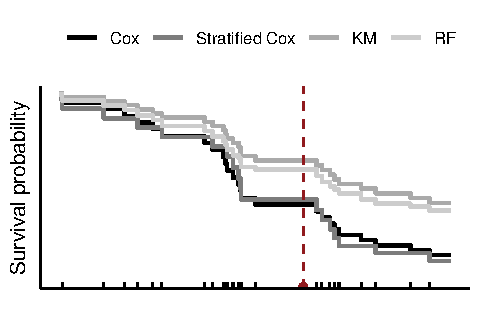
\includegraphics[width=0.8\linewidth]{sl-hold-out-sample.pdf}
% \end{center}\vspace{1cm}
% \begin{center}\vspace{1cm}
%   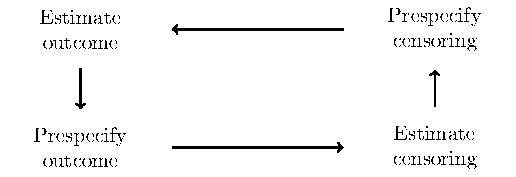
\includegraphics[width=0.6\linewidth]{ipcw-circle.pdf}  
% \end{center}\vspace{1cm}
% \end{multicols}

\section*{The state learner}

The state learner is a new super learner for survival analysis with
competing risks. The input to the state learner are libraries of
learners for all transitions of the multi-state model where censoring
is considered a state. The observed data can be regarded as
realizations of the process \( \eta(t) \in \{-1, 0, 1,2\} \) defined
by
\begin{equation*}
  \eta(t) = \1{
    \left\{
      \tilde{T} \leq t, \tilde D=1
    \right\}} + 2\,\1{\left\{\tilde{T} \leq t, \tilde
      D=2\right\}} - \1{\left\{\tilde{T} \leq t, \tilde D=0\right\}},
  \quad \text{for} \quad t \in [0, \tau].
\end{equation*}

\begin{minipage}[t]{0.5\linewidth}
  \begin{center}
    \textbf{The process \( \eta \)} \\[1em]
    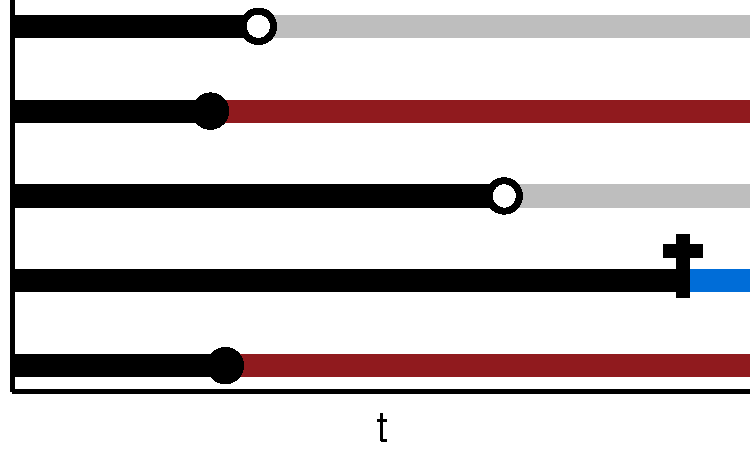
\includegraphics[width=0.8\linewidth]{multi-state-data-3.pdf}
\end{center}
\end{minipage}
\begin{minipage}[t]{.5\linewidth}
  \begin{center}
    \textbf{The states of the observed system} \\[1em]
    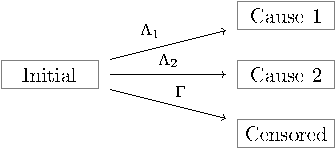
\includegraphics[width=.9\linewidth]{comp-risk-observed-w-text.pdf}
\end{center}
\end{minipage}

\vspace{1cm}

The state learner is a super learner for the conditional state-occupation
probability function, 
\begin{equation*}
  F(t, k, w,a) = P(\eta(t) = k \mid W=w, A=a).
  % \quad \text{for all} \quad
  % t \in [0,\tau],
  % k \in \{-1,0,1,2\},
  % w \in \mathcal{W},
  % a \in \{0,1\}.
\end{equation*}
Performance of a learner for \( F \) is cross-validated in the
observed data using the integrated Brier score:
\begin{equation*}
  \bar B_\tau( F,O) = \int_0^{\tau} B_t(F,O) \diff t,
  \quad \text{where} \quad 
  B_t(F,O) = \sum_{j=-1}^{2}
  \Bigl(
    F(t,j,W,A) - \1{\{\eta(t)=j\}}
  \Bigr)^2.
\end{equation*}

\section*{Building a library for state learning}

Learners of \( F \) are obtained using libraries of learners of the
cause-specific cumulative hazard functions \( \Lambda_{1} \) and
\( \Lambda_{2} \), and a library for learning the cumulative hazard of
censoring, denoted by $\Gamma$:
% Most existing survival estimators
% provide estimates of cumulative hazard functions, so these learner are
% easily available.
\begin{align*}
  F(t, 0, w,a)
  &= P{\left( \tilde{T}>t \midd W=w,A=a \right)}
  % = \Prodi_{[0,t]}
    = \Prodi_0^t
    \left( 1 - 
    \left[\Lambda_{1} + \Lambda_{2} + \Gamma
    \right](\diff s \mid w,a) \right),
  \\
  F(t, j, w,a)
  & = P{\left(
    \tilde{T} \leq t, \Delta=j \midd W=w, A=a
    \right)}
    = \int_0^t F(t-,0, w,a)  \Lambda_{j}(\diff s \mid w,a),
    \quad  j \in \{1,2\},
  \\[.7em]
  F(t, -1, w,a)
  & =
    P{\left( \tilde{T} \leq t, \Delta=0 \midd W=w, A=a \right)}
    = \int_0^tF(t-,0, w,a)  \Gamma(\diff s \mid w,a),
\end{align*}

  \section*{Theoretical and empirical results}
  \vspace{-.7em}
  \setlength{\columnseprule}{0pt} \setlength{\columnsep}{30pt}
\begin{multicols}{2}
  In \cite{munch2024} we provide a finite sample oracle inequality for the state
  learner along with other theoretical results. We confirm these results in a
  simulation study, where the state learner performs as well as a super learner
  that uses a correctly specified model to estimate inverse probability of
  censoring weights. The state learner learns the correct censoring model from
  the data at the same time as learning the outcome model. This is illustrated
  in the figure to the right.

  \vfill\null \columnbreak
  
  \begin{center}
    % {\color{white}dummy} \vspace{-10cm}
  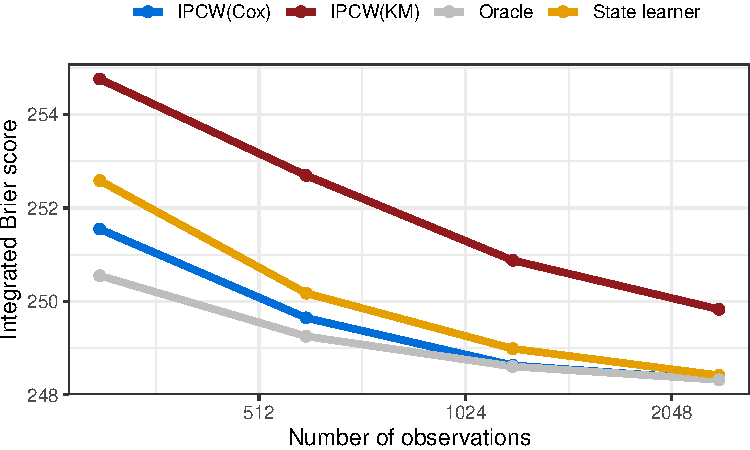
\includegraphics[width=1\linewidth]{experiment-fig-sl-ipcw.pdf} 
\end{center}

\end{multicols}

% \section*{Application}
\vspace{-1em}

\setlength{\columnseprule}{0pt}
\setlength{\columnsep}{30pt}
\begin{multicols}{2}
    %   \setlength{\parskip}{.5em}
    %   \setlength{\parindent}{0em}
  % \noindent
  % {\color{white}dummy} \vspace{0em}
  
  We apply the state learner to data from an observational prostate
  cancer study \cite{kattan2000pretreatment}. The state learner's ranking of all
  triples of learners from the provided libraries are visualized in the figure
  below. In \cite{munch2024} we show how estimators of the average treatment
  effect of hormone therapy on tumor recurrence and death can be obtained from
  the output of the state learner. The results are shown in the figure to the
  right. \vfill\null \columnbreak
\begin{center}
  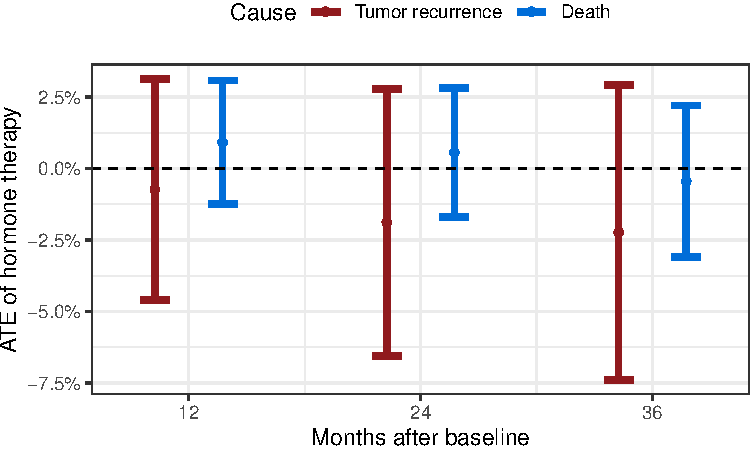
\includegraphics[width=1\linewidth]{zelefsky-data-target-par.pdf}
    % \captionof{figure}{}
    % \label{fig:zelefski-target}
\end{center}
  
\end{multicols}

% \begin{wrapfigure}{r}{0.35\linewidth}
%   \begin{center}\vspace{-1.5cm}
%     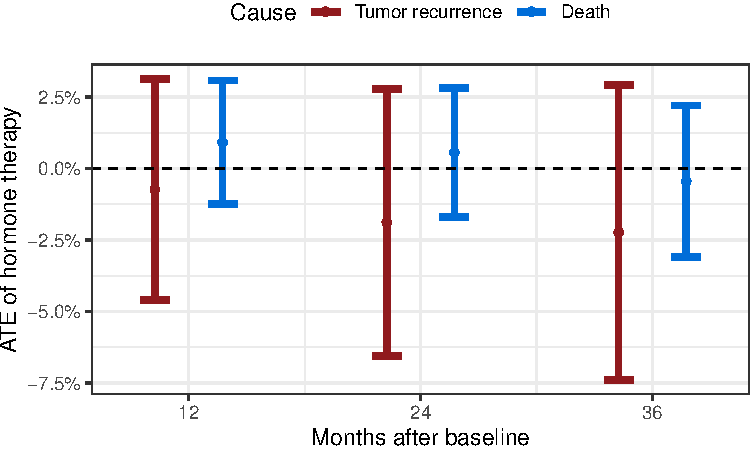
\includegraphics[width=1\linewidth]{zelefsky-data-target-par.pdf}
%     % \captionof{figure}{}
%     % \label{fig:zelefski-target}
%   \end{center}
% \end{wrapfigure}

\begin{center}
  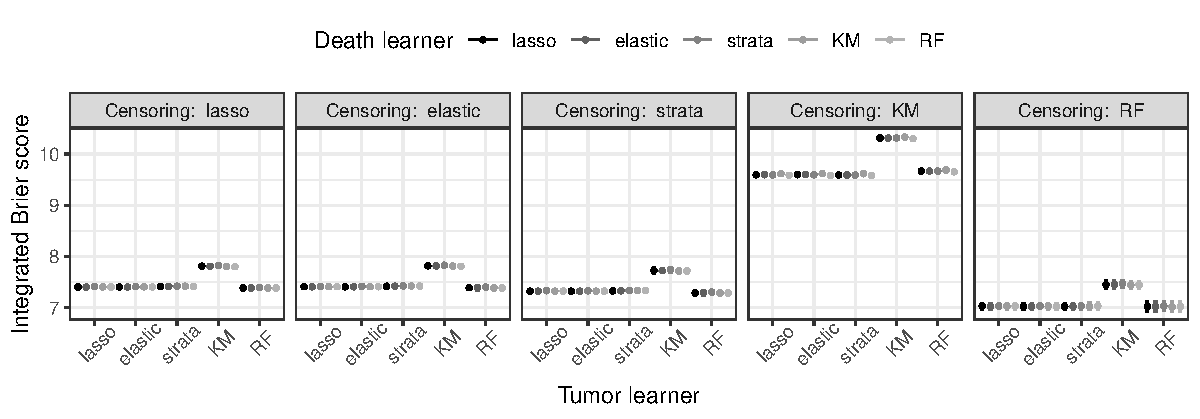
\includegraphics[width=1\linewidth]{zelefski-real-data.pdf}
  % \captionof{figure}{}
  % \label{fig:zelefski-state-learner}
\end{center}


\end{multicols}
\end{minipage}

\vspace{3em} % \vfill 

\color{DarkSlateGray} % Set the color back to DarkSlateGray for the rest of the content

% \vspace{1em}
\begin{minipage}[t]{1\linewidth}

  \setlength{\columnseprule}{0pt} \setlength{\columnsep}{30pt}

  \begin{multicols}{3}
    % [\section*{\centering \normalsize References}]
    \noindent
    
% \nocite{*} % Print all references regardless of whether they were cited in the poster or not
\bibliographystyle{plain} % Plain referencing style

\begingroup
\renewcommand{\section}[2]{}%
{\footnotesize
\bibliography{bib} }
\endgroup

\end{multicols}
\end{minipage}
\end{minipage}

\end{document}